%%%%%%%%%%%%%%%%%%%%
%     PACKAGE READERMODEL
%%%%%%%%%%%%%%%%%%%%%%%
\color{black}
\subsection{Specifica componenti Model::Util::ReaderModel}
\label{specificaReaderModel}
\begin{figure}[!h]
\centering
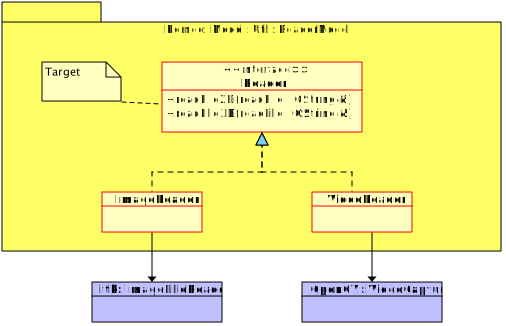
\includegraphics[scale=0.8]{../Specifica_Tecnica/Content/Immagini/Romeo__Model__Util__ReaderModel.png}
			\caption{Componente Romeo::Model::Util::ReaderModel}
			\label{comp_romeo::model::util::readermodel}
\end{figure}
Componente che contiene le classi utilizzate per leggere i vari formati di immagini su cui opera \project.

%%%%%%%%%%%%%%%%%%%%
%     INTERFACCIA READER
%%%%%%%%%%%%%%%%%%%%%%%
\subsubsection{Reader (interface)}
\label{spereader}
\begin{figure}[!h]
\centering
			\includegraphics[scale=1]{./Content/Immagini/model/Reader.png}
			\caption{Interfaccia Reader: metodi}
			\label{cl_reader}
\end{figure}
\paragraph{Descrizione \\}
L'interfaccia rappresenta un generico oggetto reader, essa fornisce il contratto ai reader concreti.
\paragraph{Utilizzo\\}
L'interfaccia fornisce dei contratti che saranno implementati dalle sottoclassi.

\paragraph{\textcolor{black}{Metodi}}
\begin{itemize}
%READFILE2D
	\item \color{blue}\verb!+ readFile2D(readFile : QString &): QVector<RGBImage2DType::Pointer>!
	\color{black}
		\subparagraph{Descrizione:} Metodo virtuale puro che ha come contratto la lettura di un file 2D. Il metodo deve essere ridefinito dalle classi che ereditano da questa, definendo la lettura di un file 2D.

		\subparagraph{Argomenti}
			\begin{itemize}
				\item \color{RoyalPurple}\verb!readFile : QString &! \\
				\color{black} Riferimento al nome del file che il metodo deve leggere.
			\end{itemize}

		\subparagraph{Note}
			\begin{itemize}
				\item questo metodo deve essere marcato virtuale puro;
				\item questo metodo deve essere ridefinito.
			\end{itemize}
%READFILE3D
	\item \color{blue}\verb!+ readFile3D(readFile : QString &): RGBImage3DType::Pointer!
	\color{black}
		\subparagraph{Descrizione:}  Metodo virtuale puro che ha come contratto la lettura di un file 3D. Il metodo deve essere ridefinito dalle classi che ereditano da questa, definendo la lettura di un file 3D.

		\subparagraph{Argomenti}
			\begin{itemize}
				\item \color{RoyalPurple}\verb!readFile : QString &! \\ 
				\color{black}Riferimento al nome del file che il metodo deve leggere.
			\end{itemize}

		\subparagraph{Note}
			\begin{itemize}
				\item questo metodo deve essere marcato virtuale puro;
				\item questo metodo deve essere ridefinito.
			\end{itemize}
\end{itemize}
\color{black}

%%%%%%%%%%%%%%%%%%%%
%     CLASSE IMAGEREADER
%%%%%%%%%%%%%%%%%%%%%%%
\subsubsection{ImageReader (class)}
\label{speimagereader}
\begin{figure}[!h]
\centering
			\includegraphics[scale=1]{./Content/Immagini/model/ImageReader.png}
			\caption{Classe ImageReader: attributi e metodi}
			\label{cl_imagereader}
\end{figure}
\paragraph{Descrizione \\}
Classe che rappresenta l'oggetto incaricato di caricare file di tipo 2D e 3D non time-dipendent.
\paragraph{Utilizzo\\}
La classe implementerà i metodi virtuali puri della superclasse. Verrà usata quando \project{} necessiterà di aver accesso alle immagini, quindi durante il salvataggio dei subject e durante l'analisi.
\paragraph{Classi ereditate\\}
	\begin{itemize}
		\item \hyperref[spereader]{Reader}.
	\end{itemize}
\paragraph{\color{black}Attributi \\}
%FOLDERNAME
	\begin{itemize}
		\item \color{blue}\verb!- static itk::ImageFileReader reader!
		\color{black}Oggetto del toolkit itk che identifica un reader per la lettura di file di tipo immagine dal file system.
	\end{itemize}
\paragraph{\textcolor{black}{Metodi}}
%costruttore
	\begin{itemize}
		\item \color{blue}\verb!+ ImageReader()!
		\color{black}
		\subparagraph{Descrizione:} Costruttore pubblico della classe ImageReader.

%READFILE2D

		\item \color{blue}\verb!+ readFile2D(readFile : QString &): QVector<RGBImage2DType::Pointer>!
		\color{black}
		\subparagraph{Descrizione:} Metodo che implementa il contratto fornito dalla classe astratta \hyperref[spereader]{Reader}. Esso restituisce un oggetto di tipo QVector di puntatori ad  RGBImage2DType, il quale rappresenta l'immagine presente nel disco al percorso indicato dal parametro readFile di tipo riferimento a QString. In questo caso il QVector sarà composto da un solo elemento. 

	\subparagraph{Argomenti}
		\begin{itemize}
			\item \color{RoyalPurple}\verb!readFile : QString &! \\
			\color{black} Riferimento al nome del file che il metodo deve leggere.
		\end{itemize}
\color{black}
	\subparagraph{Note}
		\begin{itemize}
			\item questo metodo deve essere marcato virtuale;
			\item questo metodo è stato ridefinito.
		\end{itemize} 
%READFILE3D
	\item \color{blue}\verb!+ readFile3D(readFile : QString &): RGBImage3DType::Pointer!
	\color{black}
	\subparagraph{Descrizione:} Metodo che implementa il contratto fornito dalla classe astratta \hyperref[spereader]{Reader}. Esso restituisce un oggetto di tipo puntatore ad  RGBImage3DType, il quale rappresenta l'immagine presente nel disco al percorso indicato dal parametro readFile di tipo riferimento a QString.

	\subparagraph{Argomenti}
		\begin{itemize}
			\item \color{RoyalPurple}\verb!readFile : QString &! \\ 
			\color{black}Riferimento al nome del file che il metodo deve leggere.
		\end{itemize}

	\subparagraph{Note}
		\begin{itemize}
			\item questo metodo deve essere marcato virtuale;
			\item questo metodo è stato ridefinito.
	\end{itemize} 
\end{itemize}
\color{black}
%%%%%%%%%%%%%%%%%%%%
%     CLASSE VIDEOREADER
%%%%%%%%%%%%%%%%%%%%%%%
\subsubsection{VideoReader (class)}
\label{spevideoreader}
\begin{figure}[!h]
\centering
			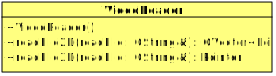
\includegraphics[scale=1]{./Content/Immagini/model/VideoReader.png}
			\caption{Classe VideoReader: attributi e metodi}
			\label{cl_videoreader}
\end{figure}
\paragraph{Descrizione \\}
Classe che rappresenta l'oggetto incaricato di caricare file di tipo 2D e 3D time-dipendent.
\paragraph{Utilizzo\\}
La classe implementerà i metodi virtuali puri della superclasse \hyperref[spereader]{Reader}. Essa verrà utilizzata quando \project{} avrà necessità di operare sui video, quindi durante il salvataggio dei subject\g{} e durante l'analisi.
\paragraph{Classi ereditate\\}
	\begin{itemize}
		\item \hyperref[spereader]{Reader}.
	\end{itemize}
\paragraph{\color{black}Attributi \\}
	\begin{itemize}
%FOLDERNAME
		\item \color{teal}\verb!- itk::VideoFileReader reader!
		\color{black}
		\subparagraph{Descrizione:} Oggetto del toolkit itk che identifica un reader per la lettura di file di tipo video dal file system.
	\end{itemize}

\paragraph{\textcolor{black}{Metodi\\}}
	\begin{itemize}
%costruttore
		\item \color{blue}\verb!+ VideoReader()!
		\color{black}
		\subparagraph{Descrizione:}Costruttore pubblico della classe VideoReader. \\

%READFILE2D
		\item \color{blue}\verb!+ readFile2D(readFile : QString &): QVector<RGBImage2DType::Pointer>!
		\color{black}
		\subparagraph{Descrizione:} Metodo che implementa il contratto fornito dalla classe astratta \hyperref[spereader]{Reader}.  Esso restituisce un oggetto di tipo QVector di puntatori ad  RGBImage2DType, il quale rappresenta i frame del video presente nel disco al percorso indicato dal parametro readFile di tipo riferimento a QString. In questo caso il QVector sarà composto da tanti elementi quanti sono i frame del video indicato.

		\subparagraph{Argomenti}
			\begin{itemize}
				\item \color{RoyalPurple}\verb!readFile : QString &! \\ 
				\color{black}Riferimento al nome del file che il metodo deve leggere.
			\end{itemize}

		\subparagraph{Note}
			\begin{itemize}
				\item questo metodo deve essere marcato virtuale;
				\item questo metodo è stato ridefinito.
			\end{itemize}
 
%READFILE3D
		\item \color{blue}\verb!+ readFile3D(readFile : QString &): RGBImage3DType::Pointer!
		\color{black}
		\subparagraph{Descrizione:} Metodo che implementa il contratto fornito dalla classe astratta \hyperref[spereader]{Reader}. Esso restituisce un oggetto di tipo puntatore ad  RGBImage3DType, il quale rappresenta il video presente nel disco al percorso indicato dal parametro readFile di tipo riferimento a QString.

		\subparagraph{Argomenti}
			\begin{itemize}
				\item \color{RoyalPurple}\verb!readFile : QString &! \\ 
				\color{black}Riferimento al nome del file che il metodo deve leggere.
			\end{itemize}

		\subparagraph{Note}
			\begin{itemize}
				\item questo metodo deve essere marcato virtuale;
				\item questo metodo è stato ridefinito.
			\end{itemize}
\end{itemize}
			\color{black}
%%%%%%%%%%%%%%%%%%%%
%     PACKAGE EXPORTERMODEL
%%%%%%%%%%%%%%%%%%%%%%%
\subsection{Specifica componenti Model::Util::ExporterModel}
\label{specificaExporterModel}
\begin{figure}[!h]
\centering
\includegraphics[scale=0.8]{../Specifica_Tecnica/Content/Immagini/Romeo__Model__Util__ExporterModel.png}
			\caption{Componente Romeo::Model::Util::ExporterModel}
			\label{comp_romeo::model::util::exporterrmodel}
\end{figure}
Componente che contiene le classi utilizzate per esportare in vari formati i risultati delle analisi effettuati da \project.

%%%%%%%%%%%%%%%%%%%%
%     INTERFACCIA EXPORTER
%%%%%%%%%%%%%%%%%%%%%%%
\subsubsection{Exporter (interface)}
\label{spexporter}
\begin{figure}[!h]
\centering
\includegraphics[scale=1]{./Content/Immagini/model/Exporter.png}
			\caption{Interfaccia Exporter: metodi}
			\label{cl_exporter}
\end{figure}
\paragraph{Descrizione \\}
L'interfaccia rappresenta un generico oggetto exporter, essa fornisce il contratto alle classi exporter concrete.
\paragraph{Utilizzo\\}
L'interfaccia fornisce dei contratti puri che saranno implementati dalle sottoclassi.
\paragraph{\textcolor{black}{Metodi\\}}
	\begin{itemize}

%READFILE2D

		\item \color{blue}\verb!+ exportImage(file : QString &, image: RGBImage*)!
		\subparagraph{Descrizione:} Metodo virtuale puro che ha come contratto la scrittura di un oggetto di tipo RGBImage su file system con il nome contenuto nel parametro file.
\color{black}
		\subparagraph{Argomenti}
			\begin{itemize}
				\item \color{RoyalPurple}\verb!file : QString &! \\ 
				\color{black}Riferimento al nome che il metodo deve dare al file che scriverà nel file system.
				\item \color{RoyalPurple}\verb!image : RGBImage*! \\ 
				\color{black}Puntatore all'oggetto che rappresenta l'immagine che il metodo deve scrivere su file system
			\end{itemize}
\color{black}
		\subparagraph{Note}
			\begin{itemize}
				\item questo metodo deve essere marcato virtuale puro;
				\item questo metodo deve essere ridefinito.
			\end{itemize}
	\end{itemize}
		\color{black}

%%%%%%%%%%%%%%%%%%%%
%     CLASSE EXPORTER2D
%%%%%%%%%%%%%%%%%%%%%%%
\subsubsection{Exporter2D (class)}
\label{spexporter2d}
\begin{figure}[!h]
\centering
			\includegraphics[scale=1]{./Content/Immagini/model/Exporter2D.png}
			\caption{Classe Exporter2D: attributi e metodi}
			\label{cl_exporter2d}
\end{figure}
\paragraph{Descrizione \\}
Classe che rappresenta l'oggetto incaricato di scrivere sul disco le immagini 2D elaborate in \project.
\paragraph{Utilizzo\\}
La classe implementerà i metodi virtuali puri della superclasse.
\paragraph{Classi ereditate\\}
\begin{itemize}
\item \hyperref[spexporter]{Exporter}.
\end{itemize}
\paragraph{\color{black}Attributi \\}
	\begin{itemize}
%FOLDERNAME
		\item \color{teal}\verb!- itk::ImageFileWriter writer!
		\color{black}
		\subparagraph{Descrizione:} Oggetto del toolkit itk che identifica un writer per la scrittura di file di tipo immagine 2D nel file system.
	\end{itemize}	
\paragraph{\textcolor{black}{Metodi}}
	\begin{itemize}
%costruttore
		\item \color{blue}\verb!+ Export2D()!
		\color{black}
		\subparagraph{Descrizione:} Costruttore pubblico della classe Export2D.

%READFILE2D

		\item \color{blue}\verb!+ ExportFileconst (file: QString&, image: RGBImage*): void RGBImage2DType::Pointer!
		\color{black}
		\subparagraph{Descrizione:} Metodo che implementa il contratto fornito dalla classe astratta \hyperref[spexporter]{Exporter}. Esso scrive su disco l'immagine rappresentata dal parametro image di tipo puntatore ad RGBImage nel percorso indicato dal parametro file di tipo riferimento a QString.

		\subparagraph{Argomenti}
			\begin{itemize}
				\item \color{RoyalPurple}\verb!file : QString &! \\ 
				\color{black}Riferimento al nome che l'immagine scritta sul disco dovrà avere.
				\item \color{RoyalPurple}\verb!image : RGBImage*! \\ 
				\color{black}Puntatore all'oggetto rappresentante l'immagine che dovrà essere scritta su disco.
			\end{itemize}
\color{black}
		\subparagraph{Note}
			\begin{itemize}
				\item questo metodo deve essere marcato virtuale;
				\item questo metodo deve essere marcato costante;
				\item questo metodo è stato ridefinito.
			\end{itemize} 
	\end{itemize}
\color{black}


%%%%%%%%%%%%%%%%%%%%
%     CLASSE EXPORTER3D
%%%%%%%%%%%%%%%%%%%%%%%
\subsubsection{Exporter3D (class)}
\label{spexporter3d}
\begin{figure}[!h]
\centering
			\includegraphics[scale=1]{./Content/Immagini/model/Exporter3D.png}
			\caption{Classe Exporter3D: attributi e metodi}
			\label{cl_exporter3d}
\end{figure}
\paragraph{Descrizione \\}
Classe che rappresenta l'oggetto incaricato di scrivere sul disco le immagini 3D elaborate in \project.
\paragraph{Utilizzo\\}
La classe implementerà i metodi virtuali puri della superclasse.
\paragraph{Classi ereditate\\}
\begin{itemize}
\item \hyperref[spexporter]{exporter}.
\end{itemize}
\paragraph{\color{black}Attributi \\}
	\begin{itemize}
%FOLDERNAME
		\item \color{teal}\verb!- itk::ImageFileWriter writer!
		\color{black}
		\subparagraph{Descrizione:} Oggetto del toolkit itk che identifica un writer per la scrittura di file di tipo immagine 3D nel file system.
	\end{itemize}
\paragraph{\textcolor{black}{Metodi}}
	\begin{itemize}
%costruttore
		\item \color{blue}\verb!+ Export3D()!
		\color{black}
		\subparagraph{Descrizione:} Costruttore pubblico della classe Export3D.

%READFILE2D

		\item\color{blue}\verb!+ ExportFileconst (file: QString&, image: RGBImage*): void RGBImage2DType::Pointer!
		\color{black}
		\subparagraph{Descrizione:} Metodo che implementa il contratto fornito dalla classe astratta \hyperref[spexporter]{Exporter}. Esso scrive su disco l'immagine rappresentata dal parametro image di tipo puntatore ad RGBImage nel percorso indicato dal parametro file di tipo riferimento a QString.

		\subparagraph{Argomenti}
			\begin{itemize}
				\item \color{RoyalPurple}\verb!file : QString &! \\ 
				\color{black}Riferimento al nome che l'immagine scritta sul disco dovrà avere.
				\item \color{RoyalPurple}\verb!image : RGBImage*! \\ 
				\color{black}Puntatore all'oggetto rappresentante l'immagine che dovrà essere scritta su disco.
			\end{itemize}
\color{black}
		\subparagraph{Note}
			\begin{itemize}
				\item questo metodo deve essere marcato virtuale;
				\item questo metodo deve essere marcato costante;
				\item questo metodo è stato ridefinito.
			\end{itemize} 
	\end{itemize}
\color{black}
